\documentclass[12pt]{article}

\usepackage{sbc-template}
\usepackage{graphicx,url}
\usepackage[utf8]{inputenc}
\usepackage[brazil]{babel}
\usepackage[latin1]{inputenc}  
\usepackage[T1]{fontenc}
\usepackage{textcomp}

\sloppy

\title{Relatório Técnico}

\author{Bonifácio de Oliveira, Lucas Araújo, Luiz Fábio, Luiz Felipe, Rafaela Melo }


\address{Escola Superior de Tecnologia -- Universidade do Estado do Amazonas
  (UEA)\\
  Manaus -- AM -- Brazil
  \email{\{bldof.eng16, lsda.lic16, lfba.lic17, lfda.lic17, rmf.lic16\}@uea.edu.br}
}

\begin{document} 

\maketitle

\begin{abstract}
This technical report describes the data analysis process for COVID-19 in Amazonas, through exploratory analysis and data visualization.
\end{abstract}
     
\begin{resumo} 
  Este relatório técnico descreve o processo de análise de dados referentes ao COVID-19 no Amazonas, por meio de análise exploratória e visualização de dados.
\end{resumo}

\section{Introdução}
O presente relatório tem como objetivo apresentar uma análise exploratória de registros de casos pessoas com COVID-19. O banco de dados utilizado\footnote{Disponível em: https://covid19.manaus.am.gov.br/wp-content/uploads/Manaus.csv} está em constante atualização, contabilizando sempre novos registros, por isto, as análises deste relatório foram realizadas com o download do banco no dia 12/08/2020. Os códigos fontes desenvolvidos são de código aberto e estão disponíveis na plataforma Github\footnote{Disponível em: https://github.com/BonifacioDeOliveira/PP1\_RNA\_UEA}. As análises foram feitas através da linguagem de programação \textit{Python}, sendo utilizadas as bibliotecas: \textit{Pandas}, para manipular os dados; \textit{Numpy}, para realizar alguns cálculos específicos; e \textit{Matplotlib} e \textit{Seaborn}, para gerar gráficos.

\section{Visão Geral dos Casos Confirmados}
% questoes 1, 2 e 3

O dataset apresenta 40 atributos, são eles: idade, faixa etária, sexo, bairro, classificacao, comorb\_renal, comorb\_diabetes, comorb\_imuno, comorb\_cardio, conclusao, dt\_notificacao, taxa, dt\_evolucao, raca, dt\_sintomas, criterio, sintoma\_garganta, sintoma\_dispneia, sintoma\_febre, sintoma\_tosse, sintoma\_outros, etnia, profiss\_saude, srag, se\_notificacao, distrito, bairro\_mapa, comorb\_respiratoria, comorb\_cromossomica, comorb\_hepatica, comorb\_neurologica, comorb\_hemato, comorb\_obessidade, origem, evolução, teste\_pcr, teste\_anticorpo, teste\_antigeno, teste\_igm e teste\_igg. Em Manaus, há 39037 casos confirmados, o caso mais antigo é datado em 01/04/2020 e o mais recente em 12/08/2020.

% questao 1

Considerando a tarefa de análise proposta, foi realizada uma limpeza nos dados retirando atributos que não influenciam nos resultados e as linhas que não continham todos os dados preenchidos. Após a limpeza e organização restaram 11 atributos e 54782 exemplos, classificados em: 14226 casos em análise, 31942 casos descartados e 8614 casos confirmados.

% questao 2, 3, 4

Os números apresentados a partir daqui são referentes ao dataset resultante após a limpeza e organização dos dados. Do total de 8614 casos confirmados, 94.87\% das pessoas se recuperaram. O número de casos no sexo feminino se sobressai ao sexo masculino, totalizando 4715 mulheres infectadas. Com relação a idade dos indivíduos contaminados, a média é 42 anos e o desvio-padrão é 15 anos, a pessoa mais jovem a contrair a doença tem 0 anos e a mais idosa 105 anos.

% questao 5, 6

O bairro com maior incidência de casos é o Cidade Nova. Os três bairros com maior número de recuperados são: Cidade Nova (371), São José Operário (321) e Flores (314). A Tabela \ref{tab1} apresenta a quantidade de testes de cada tipo e a porcentagem de cada um deles com relação ao total de 49354 testes realizados. Observa-se que o teste Anticorpo foi o mais utilizado e o IGG, o menos utilizado.

% questao 7
\begin{table}[h]\footnotesize
	\centering
	\caption{Testes Realizados}
	\begin{tabular}{|l|c|c|}
		\hline
	\textbf{Tipo de Teste}	& \textbf{Quantidade}  & \textbf{Porcentagem em relação ao total (\%)}  \\ \hline
	PCR	& 11699 & 23.7\\ \hline
	Anticorpo	& 31656  & 64.14 \\ \hline
	Antigeno	& 5905 & 11.96  \\ \hline
	IGM	& 76 & 0.15 \\ \hline
	IGG	& 18 & 0.03 \\ \hline
	\end{tabular}
	\label{tab1}
\end{table}

A taxa de letalidade calculada a partir da fração de óbitos pelo total de casos confirmados é de 5.13\%. O cálculo da correlação entre a idade e o número de casos resultou em -0.2329, uma correlação negativa fraca.


\section{Visualização de Dados}
%Questão 1
A Figura \ref{fig:seção_2.2_questão_1} apresenta um histograma informando os 10 bairros com maiores quantidades de casos registrados. A Figura \ref{fig:seção_2.2_questão_1} também indica que o bairro com maior quantidade de casos registrados foi o ``Cidade Nova''. A categoria ``Outros'' trata da soma dos bairros remanentes.

\begin{figure}[!ht]
  \centering
    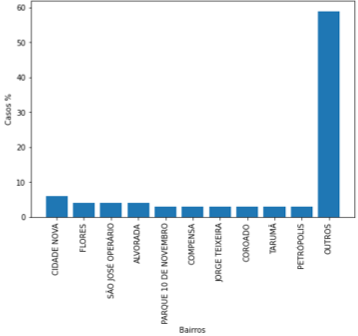
\includegraphics[width=.5\linewidth]{Figuras/porcentagem_de_casos_por_bairros.png} \\
  \caption{Porcentagem de casos por bairros.}
  \label{fig:seção_2.2_questão_1}
\end{figure}

%Questão 2
Analisando a Figura \ref{fig:seção_2.2_questão_2}, representando o \textit{boxplot} de idade com casos confirmados por sexo, é possível observa que os casos de sexo Feminino e Masculino apresentaram uma variabilidade bem similar. Além disso ambos os sexos apresentaram valores discrepante , \textit{outliers}, acima de 80 anos no sexo Masculino e um pouco abaixo também dos 80 anos no sexo Feminino, e ambas apresentaram \textit{outliers} acima de 0.

\begin{figure}[!ht]
  \centering
    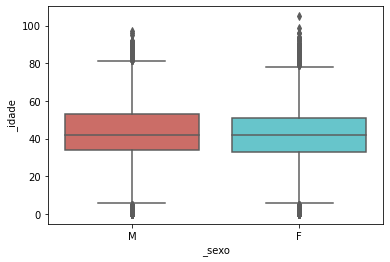
\includegraphics[width=.5\linewidth]{Figuras/boxplot_sexo_idade.png} \\
  \caption{Boxplot da idade de casos confirmado.}
  \label{fig:seção_2.2_questão_2}
\end{figure}

%Questão 3
A Figura \ref{fig:seção_2.2_questão_3} é um gráfico de barras que informa a quantidade de casos entre os períodos 03/08/2020 a 12/08/2020, mas após a limpeza dos dados, apenas duas datas foram consideradas, são elas: 04/08/2020 e 09/08/2020. A Figura \ref{fig:seção_2.2_questão_3} informa que, dentre as datas, o dia 04 foi a data com mais ocorrências (com 2 casos confirmados de COVID-19).

\begin{figure}[!ht]
  \centering
    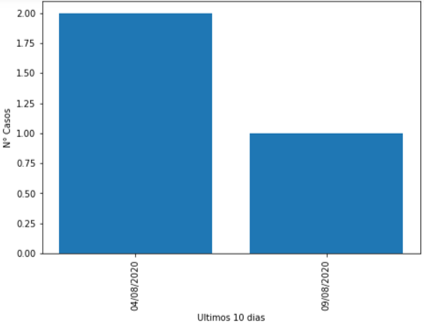
\includegraphics[width=.5\linewidth]{Figuras/numero_de_casos_nos_ultimos_10_dias.png} \\
  \caption{Porcentagem de casos por bairros.}
  \label{fig:seção_2.2_questão_3}
\end{figure}

%Questão 4
Em relação aos casos que obtiveram a conclusão igual a ``Recuperados'' durante o período entre os dias 03/08/2020 a 12/08/2020, o data set estudado não obtinha casos marcados com recuperados durante esse período. Desta forma não foi possível gerar um gráfico similar a análise anterior pois a quantidade de casos recuperados por dia entre o período citado retornava vazio.

%Questão 5
A Figura \ref{fig:seção_2.2_questão_5} informa a porcentagem de casos registrados por faixa etária (classificadas em décadas). Na Figura \ref{fig:seção_2.2_questão_5} as faixas etárias foram ordenadas de acordo com seus números de casos. É possível identificar que mais de 25\% dos casos registrados foram de pessoas entre 40 - 49 anos de idade.

\begin{figure}[!ht]
  \centering
    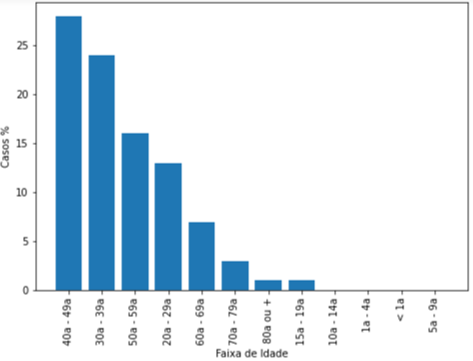
\includegraphics[width=.5\linewidth]{Figuras/casos_por_faixa_etaria.png} \\
  \caption{Porcentagem de casos por faixas etárias.}
  \label{fig:seção_2.2_questão_5}
\end{figure}

\begin{figure}[!ht]
  \centering
    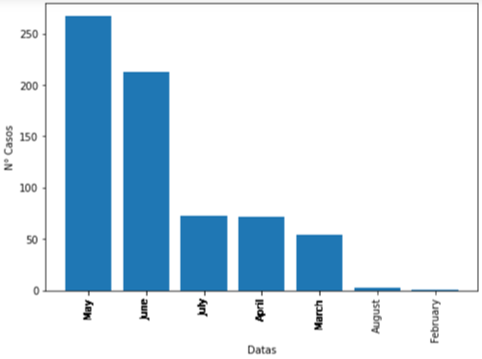
\includegraphics[width=.5\linewidth]{Figuras/casos_por_mês.png} \\
  \caption{Número de casos ao longo do tempo.}
  \label{fig:seção_2.2_questão_6}
\end{figure}

%Questão 6
A Figura \ref{fig:seção_2.2_questão_6} mostra as ocorrências de casos registrados ao longo do tempo (classificados por meses). A Figura \ref{fig:seção_2.2_questão_6} indica que ``Maio'' foi o mês com mais ocorrências registradas (mais de 250 casos).

\begin{figure}[!ht]
  \centering
    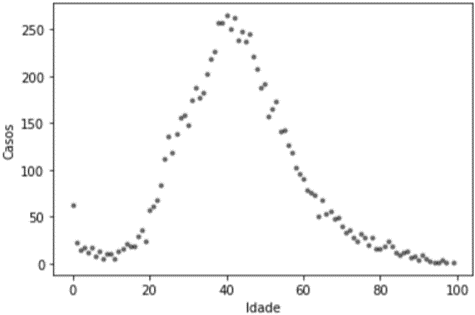
\includegraphics[width=.5\linewidth]{Figuras/casos_por_idade.png} \\
  \caption{Número de casos registrados por idade.}
  \label{fig:seção_2.2_questão_7}
\end{figure}

%Questão 7
A Figura \ref{fig:seção_2.2_questão_7} apresentada a quantidade de casos por idade, semelhante a Figura \ref{fig:seção_2.2_questão_5} que informa as faixas etárias. A Figura \ref{fig:seção_2.2_questão_7} informa que as maiores quantidade de casos foram de pessoas com idade perto dos 40 anos. É possível observar uma tendência para esta idade, visto que, as idades mais distantes dos 40 anos possuem menos casos.

\section{Tipos de Tarefas}
%Questão 1

Considerando a grande demanda de teste para a Covid-19 e o número insuficientes de testes disponíveis, umas das formas de prevenir a contaminação de outras pessoas seria levar em consideração os sintomas dos pacientes que ainda não puderam ser testados colocando-os em observação e isolamento preventivo, onde o atributo-alvo é a Classificação, para tentar prever a possibilidade uma pessoa estar contaminada ou não. Para isso seriam levados em consideração os atributos relacionados aos sintomas que o paciente apresenta como: \_sintoma\_garganta; \_sintoma\_dispneia;\_sintoma\_febre;\_sintoma\_tosse;\_sintoma\_outros;. Como métrica de desempenho a utilização da Revocação é a mais recomendada por se tratar de um diagnóstico médico visando prever uma pessoa possivelmente contaminada. O tipo de validação do modelo pode ser o K-Fold devido á grande quantidade de dados, a possibilidade de múltiplos testes e também a necessidade dos resultados do modelo serem o mais realístico possível, evitando diagnósticos incorretos.

% Questão 2
O crescente número de mortos pela Covid-19 tem criado uma crise no sistema funerário, visto que muitas agências funerárias e cemitérios não estavam preparados para um cenário tão catastrófico como esse. Para evitar o problema de falta de caixões, covas etc., a regressão poderia ser utilizada para prever o número de mortos previstos para que os agentes funerários estejam preparados e todos tenham um sepultamento digno e sem frustrações. Os atributos preditores podem ser a data de notificação, data de óbito e a evolução da doença, fazendo uma projeção do crescimento do número de mortes em um determinado tempo no futuro.

%3. Bônus: Qual tarefa de Aprendizado Não-Supervisionado poderia ser concebida neste contexto?

Na Aprendizagem supervisionado poderíamos ter como resultados a categorização dos elementos em faixas etárias, com crianças, adolescentes, adultos e idosos, sendo possível visualizar o tamanho de cada grupo.

%\bibliographystyle{sbc}
%\bibliography{sbc-template}

\end{document}
